\section{Theoretical Analysis}
\label{sec:analysis}

In this section, the circuit shown in Figure~\ref{fig:rc} is analysed
theoretically, in terms of the voltages and current intensities in the various branches and components of the circuit.

For a question of convenience and coherence

\subsection{______}

The circuit consists of multiple loops with various values of current, $i$, circulating in each of the branches of the circuit. There are two
voltage sources, $v_a$ and $v_c$, driving their inputs. Applying the Mesh Method, we reach a system of 5 equations and 5 unkowns, that we solved in Octave, after transforming the system into a matrix. Those equations are:

begin{equation}
  v_a - R_1 i_a - R_3(i_a + i_b) - R_4(i_a +i_c) = 0.
\end{equation}

$v_c - R_4(i_a +i_c) - (R_6 +R_7)i_c = 0$
$v_c = K_c i_c$
$v_b = R_3(i_a + i_b)$
$i_b = K_b v_b$

Another way of solving the circuit is the Nodal Method, in which we have reached a system of 11 equations and 11 unknowns. After obtaining the equations, we repeated the procedure we took with the Mesh Method and solved the system with Octave software. The equations obtained by this method are:

\begin{equation}
  (v_3 - v_5)G_3 + (v_3 - v_2)G_1 + (v_3 - v_4)G_2 = 0.
  \label{eq:kvl}
\end{equation}

\begin{equation}
  (v_4 - v_3)G_2 - i_b = 0.
\end{equation}

\begin{equation}
  i_b - i_d + (v_6 - v_5)G_5 = 0.
  \label{eq:kvl2}
\end{equation}

$i_b = K_b v_b$
$v_3 -v_5 = v_b$
$v_1= 0$
$v_2 - v_1 = v_a$
$v_5 - v_9 = v_c$
$v_c = K_c I_c$
$v_9 - v_1 = -i_c(r_6 + r_7)$
$(v_2 - v_3)G_1 + i_c +(v_1 - v_5)G_4 = 0$

Equation~(\ref{eq:kvl2}) 

\begin{equation}
  v_O(t) = v_{On} + v_{Of}.
  \label{eq:vo_sol}
\end{equation}

As learned in the theory classes the natural solution is of the form
\begin{equation}
  v_{On}(t) = Ae^{-\frac{t}{RC}},
  \label{eq:vo_nat}
\end{equation}
where $A$ is an integration constant.

The forced solution is of the form given in Equation~(\ref{eq:vo_for}) and is
illustrated in Figure~\ref{fig:forced}.

\begin{equation}
  
  \label{eq:vo_for}
\end{equation}

\begin{figure}[h] \centering
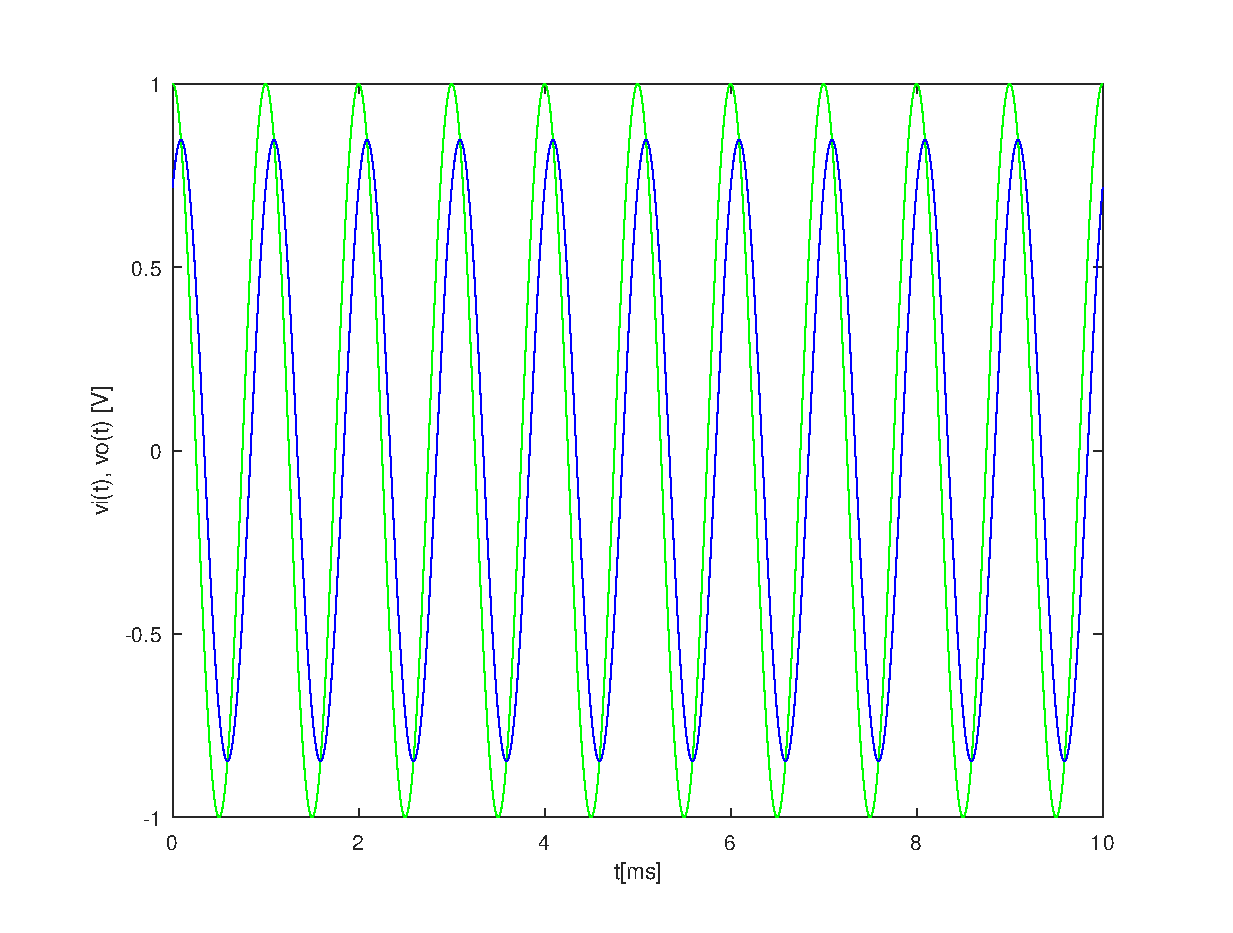
\includegraphics[width=0.8\linewidth]{forced.eps}
\caption{------------}
\label{fig:forced}
\end{figure}
